\documentclass[10pt,a4paper]{article}
\usepackage[margin=2.2cm]{geometry}
\usepackage{amsmath,amssymb}
\usepackage[T1]{fontenc}
\usepackage{lmodern}   % scalable CM clone: microtype's font expansion needs
                       % outline fonts, and the bitmap CM set isn't installed
\usepackage{microtype}
\usepackage{graphicx}
\usepackage[hidelinks]{hyperref}

\newcommand{\Lt}{L}                      % torso scale
\newcommand{\conf}{c}
\setlength{\parskip}{2pt}

\title{\textbf{coach}: pose-based technique diagnostics for weightlifting}
\author{Noah Stauble}
\date{September 2026}

\begin{document}
\maketitle
\vspace{-1.2em}
\begin{abstract}
\noindent
\texttt{coach} takes a phone video of a snatch or clean, runs top-down 2D pose
estimation over every frame, and turns individual coaching cues into scalars
computed from the resulting keypoint track. This note records the model, the
deployment, the temporal filtering applied to the track, and the geometry of
each implemented diagnostic. Every threshold below is provisional: none has
been fitted to labelled lifts. Figures are produced by \texttt{analysis.ipynb}
from one example clip (\texttt{examples/athlete-a-trim.mp4}, 107 frames at
30\,fps) through a line-for-line Python port of the browser code.
\end{abstract}

\section{Model}

Pose estimation is two-stage (top-down). A YOLOv8-s detector~\cite{yolov8}
proposes person boxes at $320\,\mathrm{px}$ input; each box is cropped, resized
and passed to ViTPose~\cite{vitpose}.

ViTPose is deliberately architecture-poor: a \emph{plain} ViT
backbone~\cite{vit} (non-hierarchical, no cross-window attention), MAE
pretrained~\cite{mae}, followed by a lightweight decoder. The crop is split into
$16\times16$ patches, embedded, and processed by $N$ standard transformer blocks
($N=24$, $d=1024$ for ViT-L; $N=32$, $d=1280$ for ViT-H --- \texttt{coach} ships
both, defaulting to L). The decoder is two deconvolution blocks (each
$2\times$ upsampling, followed by BN and ReLU) and a $1\times1$ convolution,
producing $K=17$ COCO keypoint heatmaps $H_k\in\mathbb{R}^{h/4\times w/4}$. The
prediction for joint $k$ is
\[
  \hat{u}_k=\arg\max_{u} H_k(u),
  \qquad
  \conf_k=H_k(\hat{u}_k)\in[0,1],
\]
mapped back through the crop transform to image coordinates. The confidence
$\conf_k$ is used downstream as a hard gate at $\tau=0.3$ and as a weight in the
temporal filter (\S\ref{sec:smooth}). The paper's point is that this minimal
decoder over a plain, MAE-pretrained ViT matches heavily engineered pose
architectures; the practical consequence here is that the model is a single
forward pass with no temporal prior whatsoever --- every frame is estimated
independently, which is the entire reason \S\ref{sec:smooth} exists.

For video, the SORT tracker~\cite{sort} keeps person ids stable across frames.
\texttt{coach} then discards every track but one, choosing
\[
  \hat{p}=\arg\max_{p}\Bigl(\,n_p,\ \textstyle\sum_{f}\sum_{k}\conf_{k}^{(p,f)}\Bigr)
  \quad\text{lexicographically},
\]
i.e.\ longest-lived track, ties broken on total confidence. Longevity is the
right discriminator: the lifter is in frame for the whole clip because the clip
exists to show the lift, whereas passers-by and bodies hallucinated out of
racked plates flicker. The known failure --- SORT splitting one lifter into two
ids across an occlusion --- is reported rather than hidden: dropped tracks and
their frame counts are returned in the response metadata.

\section{Website}

Flask~+~waitress on \texttt{:8080} behind Caddy (local CA, tailnet-only, no
application auth). The model loads in-process rather than behind a sidecar
service: a single YOLO~+~ViT forward pass has no queue and no per-session state
to manage, so an HTTP hop would buy nothing. Checkpoints are lazily loaded per
size and stay resident ($\approx$1.2\,GB for L, 2.5\,GB for H on a W7800 via
ROCm).

\texttt{POST /api/pose/video} returns JSON --- keypoints per processed frame,
plus \texttt{fps}, true frame count (counted while decoding, not read from
container metadata, which is unreliable for MediaRecorder output), per-frame
presentation timestamps, and the skeleton edge list. No annotated video is
encoded server-side: the box has no licensed H.264 encoder, so the browser plays
the original file it already holds and draws the skeleton on a \texttt{<canvas>}
synced to \texttt{currentTime}. All smoothing, plotting and diagnostic scoring
run client-side on the returned track, so the smoothing width is a slider rather
than a re-run.

\section{Smoothing}\label{sec:smooth}

\subsection{Confidence-weighted Gaussian in time}

Let a single keypoint's trajectory be $\mathbf{p}_k\in\mathbb{R}^2$ observed at
sample times $t_k$ with confidences $\conf_k$. The first pass is
\[
  \tilde{\mathbf{p}}_k=\frac{\sum_{j\in\mathcal{N}_k} w_{jk}\,\mathbf{p}_j}{\sum_{j\in\mathcal{N}_k} w_{jk}},
  \qquad
  w_{jk}=\exp\!\Bigl(-\tfrac{(t_j-t_k)^2}{2\sigma^2}\Bigr)\,\conf_j,
  \qquad
  \mathcal{N}_k=\{j: |t_j-t_k|\le 3\sigma,\ \conf_j\ge\tau\}.
\]
Three properties are deliberate. (i) The kernel is in \emph{time}, not in
sample index: under variable frame rate or a frame stride $>1$ a fixed sample
window is a different number of seconds at different points in the clip, and one
slider position would mean different filtering per video. (ii) Sub-threshold
neighbours are excluded and the rest weighted by $\conf_j$, so a wrist the model
guessed at while occluded does not drag its neighbours. (iii) The smoothed point
inherits its \emph{own} frame's confidence, $\tilde{\conf}_k=\conf_k$: smoothing
moves points that were already visible and never conjures a joint the gate was
hiding. Truncation at $3\sigma$ costs $<1.2\%$ of kernel mass.

\subsection{The velocity filter}

Convolution commutes with differentiation, so smoothing positions smooths
velocity by exactly the same kernel: $\widetilde{\dot{\mathbf{p}}}=g_\sigma*\dot{\mathbf{p}}$.
The Gaussian's transfer function is
\[
  \hat{g}_\sigma(f)=\exp(-2\pi^2\sigma^2f^2),
\]
so at $\sigma=50\,\mathrm{ms}$ a speed feature at $5\,\mathrm{Hz}$ (a
$200\,\mathrm{ms}$ event --- i.e.\ the second pull, or the turnover) retains only
$\exp(-1.23)\approx29\%$ of its amplitude. The lift comes out slower and more
drawn-out than it was. The smoothed \emph{path} is fine; it is the timing along
it that has been blurred.

The second pass therefore keeps the path and re-times the points along it. Let
$P_m$ be the smoothed polyline and $R_m$ the raw track over the same times.
Define cumulative arc length and unit tangents
\[
  A_m=\sum_{i\le m}\lVert P_i-P_{i-1}\rVert,
  \qquad
  \hat{T}_m=\frac{P_m-P_{m-1}}{\lVert P_m-P_{m-1}\rVert},
\]
and the raw track's \emph{progress along that path}, its frame-to-frame
displacement projected onto the tangent:
\[
  \Pi_m=\sum_{i\le m}\bigl\langle R_i-R_{i-1},\ \hat{T}_i\bigr\rangle,
  \qquad
  e_m=\Pi_m-A_m .
\]
Projection is what makes $\Pi$ usable: jitter perpendicular to the path is not
motion along it and is discarded, while jitter along the path telescopes in the
sum, so $\Pi$ is not a random walk. The residual $e_m$ is how far ahead the raw
track is at sample $m$; the corrected point is the point at arc length
$A_m+e_m$.

$e$ is band-passed before use, as a difference of two Gaussians,
\[
  \hat{e}=g_{\sigma/2}*e\;-\;g_{4\sigma}*e,
  \qquad
  s_m=\mathrm{clip}\bigl(A_m+\hat{e}_m,\ 0,\ A_{n-1}\bigr),
\]
and $Q_m$ is $P$ evaluated at arc length $s_m$ by linear interpolation within
the containing segment. Both cutoffs carry an argument:
\begin{itemize}\itemsep1pt
\item \textbf{High-frequency removal ($\le\sigma/2$).} Wobble in $e$ at frame
  scale is the raw jitter's along-path component. Handing it back would undo the
  smoothing along the tangent direction. What is restored is the shape of the
  speed profile at the timescale the Gaussian damaged, not per-frame noise.
\item \textbf{Low-frequency removal ($\ge4\sigma$).} At a sharp reversal the
  smoothed path genuinely cuts the corner and is shorter than the raw one, so
  $e$ gains that shortfall going in and again coming out, permanently. Left in,
  every reversal would shove all later points forward along the path;
  high-passed, it becomes a local correction that keeps speed up into and out of
  the corner.
\end{itemize}
The limit is structural and worth stating: speed at the apex of a cut corner
cannot be restored by reparametrizing a curve that no longer reaches it. In
exchange, the pass is a pure reparametrization --- $Q$ never leaves the smoothed
polyline, so it cannot invent a position the smoothing did not already propose.

Fig.~\ref{fig:smooth} shows both passes on the example clip's wrist. Inside
the pull the raw peak speed is $9.2\,\Lt/\mathrm{s}$; the Gaussian alone leaves
$3.3$ ($36\%$), the retiming brings it back to $5.2$ ($56\%$). The bottom panel
is the reason for the low-frequency cut: $e$ steps up by $\approx200\,\mathrm{px}$
at the turnover --- the corner the smoothed path cut --- and stays there, while
the band-passed $\hat{e}$ that is actually applied returns to zero.

\begin{figure}[t]
  \centering
  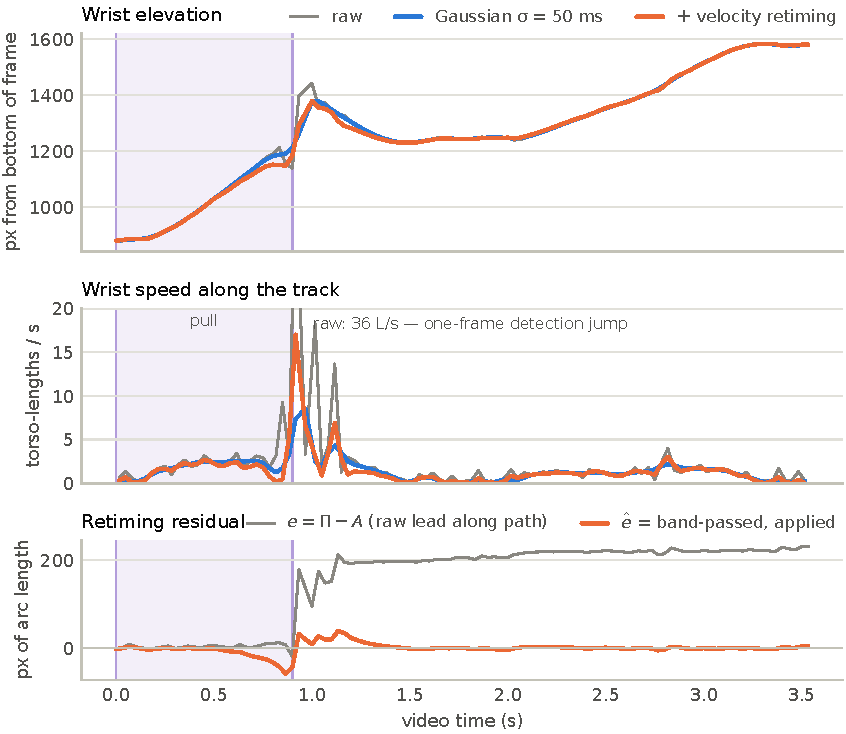
\includegraphics[width=\textwidth]{figures/smoothing.pdf}
  \caption{Temporal smoothing on one wrist keypoint, $\sigma=50\,\mathrm{ms}$.
  Top: elevation --- the retimed track lies on the Gaussian path but reaches
  each height at the raw track's time. Middle: speed along the track; the raw
  spike at the turnover is a one-frame detection jump, not motion. Bottom: the
  retiming residual $e=\Pi-A$ and its band-passed form $\hat{e}$. Purple band:
  the pull (first-pull start to second-pull end).}
  \label{fig:smooth}
\end{figure}

\subsection{Render-time interpolation}

The overlay is evaluated at the playhead's continuous time, not at the nearest
sampled frame. Interpolation is monotone cubic Hermite on uneven knots: on
$[t_1,t_2]$ with $h=t_2-t_1$, $d=(v_2-v_1)/h$,
\[
  v(u)=(2u^3-3u^2+1)v_1+(u^3-2u^2+u)h\,m_1+(-2u^3+3u^2)v_2+(u^3-u^2)h\,m_2 ,
\]
with tangents from the three-point slope, Fritsch--Carlson limited~\cite{fc}:
\[
  m=\frac{d_A h_B+d_B h_A}{h_A+h_B},\qquad
  |m|\le 3\min(|d_A|,|d_B|),\qquad
  m=0 \text{ if } d_A d_B\le 0 .
\]
Linear interpolation is $C^0$ but not $C^1$, so the mesh changes direction at
every sample --- the same stepping the interpolation is meant to remove.
Clamping matters for exactly the moments a lift is judged on: an unclamped
spline overshoots the turnaround at the bottom of a squat and draws the athlete
deeper than any frame shows them. Zeroing the tangent at a local extremum keeps
the curve inside its samples, so interpolation cannot invent a new depth, a new
lockout, or a new peak speed. Neighbours below $\tau$ do not shape the curve,
and a joint confident on only one side of a gap is not blended at all --- the
nearer sample stands until $u=0.5$.

\subsection{Preparation for scoring, and scale}

Inside \texttt{diagnostics.js} the gated track is \emph{not} smoothed again.
Holes left by the gate are filled by a 5-sample centred mean of whichever
neighbours survive, and filled points are flagged so the transparency block can
count them; they are not measurements. A second smoothing pass here would
silently mute the user's slider, since a fixed 5-frame mean removes most
per-frame jitter on its own.

All pixel thresholds are normalized by a body scale --- the median hip-to-shoulder
distance over the clip,
\[
  \Lt=\operatorname{median}_k \tfrac{1}{|S_k|}\textstyle\sum_{s\in S_k}\lVert \mathbf{p}^{\,\mathrm{hip}}_{s,k}-\mathbf{p}^{\,\mathrm{sho}}_{s,k}\rVert ,
\]
so a threshold survives the lifter standing closer to the camera. There is no
metric scale anywhere: everything is pixels in the image plane, which also means
every angle below assumes a side-on camera.

\section{Diagnostics}

A diagnostic maps one coaching cue to one scalar, and is written in three parts:
the cue and its scalar; an \emph{active phase} defined by triggers computable
from keypoints; and a visualization plus everything needed to distrust it.
Scoring a cue outside its phase is noise --- the back angle is \emph{supposed}
to change once the bar passes the knee.

Two conventions are shared. Keypoints are $[y,x,\conf]$ with $y$ growing
downward, so ``$A$ above $B$'' is $y_A<y_B$. And every measurement is computed
twice from disjoint keypoints (left side, right side); their mean is the reported
value and $|\theta_L-\theta_R|$ is the plotted uncertainty band. A persistent
L/R offset means the camera is not square (real signal); a jittery one means the
pose track is unreliable.

Two derived quantities recur. There is no bar keypoint in COCO-17, so the bar is
estimated from the hand wrapping it,
\[
  \mathbf{b}=\Bigl(x_w,\; y_w+\tfrac{1}{6}\lVert \mathbf{p}_w-\mathbf{p}_e\rVert\Bigr),
\]
averaged over visible sides ($w$ wrist, $e$ elbow). And wrist-centroid speed is
measured on a 9-sample centred mean $\bar{c}$ over a $\pm2$-sample baseline,
\[
  v_i=\frac{\lVert \bar{c}_{i+2}-\bar{c}_{i-2}\rVert}{(t_{i+2}-t_{i-2})\,\Lt}
  \quad[\Lt/\mathrm{s}],
\]
for signal-to-noise reasons: a few px of per-frame jitter over $1/30\,\mathrm{s}$
reads as $\approx0.5\,\Lt/\mathrm{s}$, several times the onset threshold, so a
one-frame difference finds ``motion'' in a lifter standing perfectly still. Over
the wider baseline the same jitter lands near $0.07$ while a real pull runs
$\approx2$. Every threshold crossing must additionally hold for $R=3$ consecutive
samples before it counts.

\subsection{Snatch}

\subsubsection{First pull --- constant back angle (implemented)}

\emph{Cue:} through the first pull the trunk keeps its inclination to the floor;
the knees open and the bar rises, but the back angle holds.

\emph{Phase:} floor to bar-past-knee. The phase is anchored on its \emph{end},
a crisp geometric crossing: the first $i$ with $b_y(i)<y_{\text{knee}}(i)$
holding for $R$ samples, scanned from the first sample where the bar is
genuinely below the knee. The start is then searched \emph{backwards} for the
last window of $R$ samples with $v<0.15\,\Lt/\mathrm{s}$. Searching forwards
from frame 0 finds the setup instead --- grip adjustments, the hook re-set and
rocking into position all clear a motion threshold before the pull starts. If no
stillness is found the start clamps to frame 0 and says so.

\emph{Measure:} the trunk's inclination to the floor, per side,
\[
  \theta=\operatorname{atan2}\bigl(y_{\text{hip}}-y_{\text{sho}},\ |x_{\text{sho}}-x_{\text{hip}}|\bigr),
\]
$0^\circ$ horizontal, $90^\circ$ vertical. The absolute value on $\Delta x$ makes
this independent of facing, so left- and right-facing videos score alike.
Reported: $\mathrm{SD}(\theta)$ over the phase (the verdict, bands
$2.5^\circ/5.0^\circ$), and drift $\Delta=\theta_{\text{end}}-\theta_{\text{start}}$,
which drives the colour ramp as $t=\min(1,|\Delta|/90^\circ)$. The cue is about
\emph{holding}, so nothing is coloured by the absolute angle: a lifter setting up
at $25^\circ$ and one at $45^\circ$ are both correct. Colour is one constant per
lift, not per frame --- recolouring frame by frame made the mark flicker through
the ramp and invited reading a single frame as a verdict. A trunk mean above
$75^\circ$ triggers a warning that the clip is filmed front-on, where the angle
saturates and the score is meaningless.

Fig.~\ref{fig:fp} is the example clip. It starts mid-pull: no still window
precedes the bar/knee crossing, so the start clamps to frame 0 and the
diagnostic says so --- a $0.47\,\mathrm{s}$ window over which the trunk drops
from $62^\circ$ to $32^\circ$ ($\Delta=-30.5^\circ$, $\mathrm{SD}=11.8^\circ$,
L/R disagreement $4.5^\circ$).

\begin{figure}[t]
  \centering
  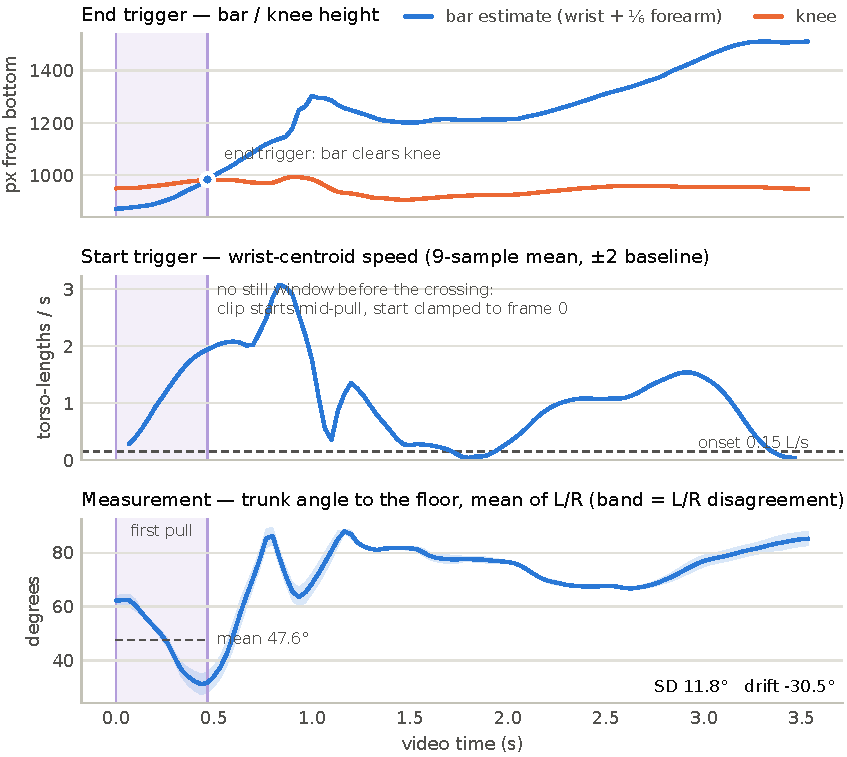
\includegraphics[width=\textwidth]{figures/first-pull.pdf}
  \caption{First pull on the example clip. Top: the two heights the end
  trigger compares; the phase ends where the bar estimate first clears the knee
  for $R$ samples. Middle: the wrist-centroid speed the start trigger searches
  backwards through. Bottom: trunk angle, mean of the two sides, band
  $=|\theta_L-\theta_R|$; SD and drift are read inside the band only.}
  \label{fig:fp}
\end{figure}

\subsubsection{Second pull --- full triple extension (implemented)}

\emph{Cue:} at the top of the second pull the hips and knees open fully before
the arms bend into the turnover.

\emph{Phase:} bar-past-knee to peak hip elevation. The start is the
\emph{same computation} that ends the first pull --- one event, computed once, so
two triggers cannot drift apart. The end is a smoothed extremum rather than a
crossing, so it needs confirmation: the running minimum of the smoothed hip
elevation counts as the peak only once the hip has given back
$\ge0.08\,\Lt$ and held that for $R$ samples. A clip ending at peak extension
reports the best point found, flagged unconfirmed.

\emph{Measure:} interior joint angles via the normalized dot product,
\[
  \angle(j;a,b)=\arccos\frac{\langle a-j,\ b-j\rangle}{\lVert a-j\rVert\,\lVert b-j\rVert},
\]
which needs no reference axis (unlike $\theta$ above) and is therefore the right
measure for a joint rather than a segment's tilt; $180^\circ$ is a straight, fully
extended joint. Hip is $\angle(\text{hip};\text{sho},\text{knee})$, knee is
$\angle(\text{knee};\text{hip},\text{ankle})$, each per side. Peak values are the
mean of the last $3$ samples of the phase, since the phase end itself came from
a smoothed signal. Deficits $\delta=180^\circ-\text{peak}$ give the verdict
(bands $10^\circ/20^\circ$) and the ramp,
\[
  t=\min\bigl(1,\ \max(\delta_{\text{hip}},\delta_{\text{knee}})/45^\circ\bigr),
\]
worst-joint, because triple extension is not met by extending only the hip.
Synchrony is reported alongside as $|t^*_{\text{hip}}-t^*_{\text{knee}}|$: the cue
names a simultaneous event, so a lifter who extends the knees well before the
hips has split it even if each joint individually reaches a good angle.

\emph{Known gap:} ankle plantarflexion is not measured. COCO-17 has no foot
keypoint, so only two of the three joints in ``triple extension'' are scored.

On the example clip (Fig.~\ref{fig:sp}) the peak is confirmed, the hip ends
$14.3^\circ$ and the knee $20.7^\circ$ short of straight (verdict: partial),
and the knee peaks $67\,\mathrm{ms}$ before the hip.

\begin{figure}[t]
  \centering
  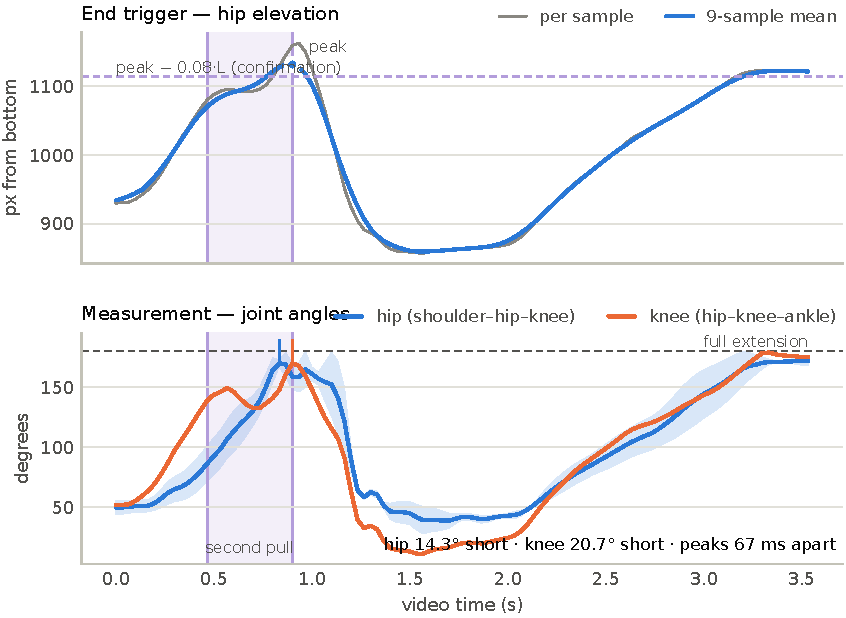
\includegraphics[width=\textwidth]{figures/second-pull.pdf}
  \caption{Second pull on the example clip. Top: hip elevation per sample and
  its 9-sample mean, on which the peak is found and confirmed once the hip gives
  back $0.08\,\Lt$. Bottom: hip and knee interior angles against the
  $180^\circ$ reference; band $=$ L/R hip disagreement; ticks at the top mark
  each joint's own peak.}
  \label{fig:sp}
\end{figure}

\subsubsection{Turnover and receiving (not implemented)}

Candidate triggers exist in the same vocabulary --- elbow angle leaving
$180^\circ$ for the turnover, the bar's vertical velocity zero-crossing, hip
elevation's second minimum for the catch --- but nothing is written yet, and no
number is shown for this window.

\subsection{Clean}

The two diagnostics above are lift-agnostic as written: both triggers (bar
crossing knee height, peak hip elevation) and both measurements (trunk
inclination, hip/knee joint angles) are grip-independent, so a clean is scored
today by the same code as a snatch. The wider grip of the snatch changes the bar
height at the crossing but not the geometry of the trigger.

What is \emph{not} covered is everything after the pull: the rack position, the
elbow whip, and the front-squat recovery have no diagnostic. Racking in
particular would need the bar estimate to survive the wrist rotating under the
bar, which the current $\tfrac{1}{6}$-forearm offset does not model.

\subsection{Jerk}

Not implemented.

\section*{Caveats}

Every band in this note ($2.5^\circ/5.0^\circ$ SD, $10^\circ/20^\circ$ short of
extension, $0.15\,\Lt/\mathrm{s}$ onset, $0.08\,\Lt$ peak confirmation) is
provisional and was set by inspection, not fitted to labelled lifts. All angles
are in the image plane and assume a side-on camera. Widening the smoothing
$\sigma$ lowers the first pull's SD whether or not the back angle actually held,
so lifts are only comparable at one setting --- which is why the applied
$\sigma$ is printed with every score.

\appendix

\section{Depth from a single view}\label{sec:depth}

Everything above is planar: ViTPose returns $(x,y)$ and the diagnostics measure
angles in the image. The 3D viewer needs a $z$ per joint, and one uncalibrated
camera does not supply one. This appendix is the geometry used to invent it,
the ambiguity that survives, and --- \S\ref{sec:depth-broken} --- what the two
errors it used to make cost, since both shaped the method that replaced them.
Implementation: \texttt{src/depth\_backend.py}.

\subsection{Foreshortening}\label{sec:depth-fore}

Take a bone whose true 3D length $L$ is known and whose endpoints project to a
screen separation $\ell$. Under an orthographic camera the screen length is the
projection of the bone onto the image plane, so the out-of-plane extent follows
from Pythagoras (Fig.~\ref{fig:depthgeom}a):
\[
  dz=\sqrt{\max(L^2-\ell^2,\,0)}.
\]
A bone of fixed length that looks short is pointing at the camera, and the
shortfall is the depth. The clamp handles $\ell>L$ --- a wrong prior or a bad
keypoint --- by placing the joint flat rather than failing.

Joints are placed by walking outward from the trunk, each child taking its
parent's depth plus its own $dz$, so flipping a forearm swings the wrist about
the elbow instead of translating the whole arm. The priors $L$ are population
anthropometry expressed in torso lengths (pelvis-to-neck $=1$): thigh and shank
$0.85$, upper arm $0.62$, forearm $0.50$.

The head is not walked. COCO gives five head keypoints; the lift carries one,
at the midpoint of the two eyes, and the nose, ears and eyes are dropped. Five
points inside a head's width resolve nothing at this scale, and they accounted
for four of the depth directions the interface asked the user about. Reaching
that point from the neck with a fixed prior would be wrong in the same way the
scale below is: neck-to-eyes is not rigid, because the athlete looks down
through the pull, and on the example clip it projects to $0.37\,\Lt$ at the
median against $0.59$ at its longest. A prior long enough to cover the $0.59$
would invent $\sqrt{0.62^2-0.37^2}=0.50\,\Lt$ of depth at a typical frame. The
head point lies on the body's sagittal midline instead, where $z=0$ holds by
construction --- so it needs no prior and has no sign to choose, and it follows
the trunk.

The torso length they are scaled by must be one number for the clip, not the
pelvis-to-neck distance measured on each frame. That distance is itself a
projection: on the example lift it runs $141\,\mathrm{px}$ at the bottom of the
pull against $251$ stood up, a factor of $1.78$, while the athlete's torso
plainly does not change length. Using the per-frame value shrinks every bone
prior by that factor exactly when the pose is most foreshortened --- and only
the priors, since $x$ and $y$ stay in real pixels --- so the recovered $z$ is
scaled by the foreshortening of a different body part. Because a projection is
never longer than what it projects, the per-frame values are all lower bounds on
one fixed quantity and the largest is the estimate; the code takes the 95th
percentile, the top of that distribution being keypoint noise.

\subsection{Scale}

The lift needs $L$ in the same units as $\ell$. Two sources, in order of
preference:

\emph{Metric, from the equipment.} A bumper plate is a $450\,\mathrm{mm}$ disc,
and a circle seen at an angle $\alpha$ to the camera projects to an ellipse
whose minor axis is foreshortened and whose major axis is not
(Fig.~\ref{fig:depthgeom}c). Fitting that ellipse gives the scale and the tilt
at once,
\[
  s=\frac{225\,\mathrm{mm}}{\mathrm{major}/2}\quad[\mathrm{mm/px}],
  \qquad
  \cos\alpha=\frac{\mathrm{minor}}{\mathrm{major}},
\]
and since the plate's normal is the bar's axis, the same fit orients the bar in
3D. This is the only true metric anchor in the system: one frame fixes both a
real distance and a real direction. It is also the only path that requires the
equipment detector, and it degrades to the alternative when no plate is found.

\emph{Relative, from the body.} Otherwise $\Lt$ (\S\ref{sec:smooth}) is the
unit and the reconstruction is in torso lengths --- enough for shape and
angles, not for measurements.

\subsection{The trunk is not a flat plate}

Shoulders and hips were originally pinned to $z=0$, which asserts the trunk is
parallel to the screen. Filmed side-on that is false and the error is not
small: on the example clip the shoulders project $0.43\,\Lt$ apart against a
true width near $0.85\,\Lt$. The same relation as
\S\ref{sec:depth-fore} applies to a left/right pair of known width $W$ and
observed separation $d$,
\[
  dz_{\text{pair}}=\tfrac{1}{2}\sqrt{\max(W^2-d^2,\,0)},
\]
applied with opposite signs to the two sides so the trunk turns about its own
axis rather than the body sliding in depth. Shoulders and hips share one sign:
independent signs would permit a $180^\circ$ twist between hip and shoulder. The
cost is that real, modest torso twist is not modelled.

\begin{figure}[t]
  \centering
  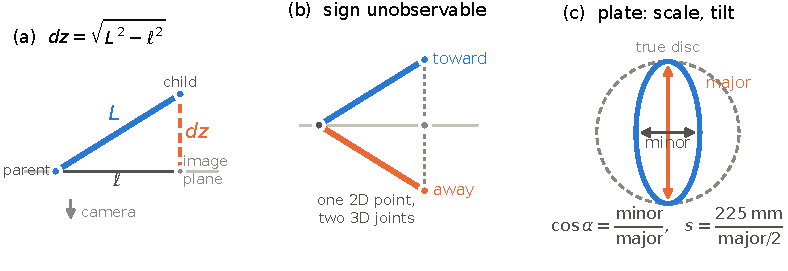
\includegraphics[width=\textwidth]{figures/depth-geometry.pdf}
  \caption{The three pieces of geometry, all seen from above. (a) A bone of
  known length $L$ measured at screen length $\ell$ spends the difference in
  depth. (b) The same triangle has two solutions --- toward the camera and away
  --- projecting to the identical 2D point; one unobservable bit per joint.
  (c) A plate is a circle of known diameter, so its fitted ellipse yields the
  metric scale $s$ and the tilt $\alpha$ of the bar out of the image plane.}
  \label{fig:depthgeom}
\end{figure}

\subsection{The sign ambiguity}\label{sec:depth-sign}

$dz$ has a magnitude but no sign: an elbow foreshortened by $30\,\mathrm{px}$ is
equally consistent with bending toward the camera or away from it
(Fig.~\ref{fig:depthgeom}b). Both reconstructions fit the image \emph{exactly},
so no amount of 2D evidence separates them, and with $n$ such joints there are
$2^n$ reconstructions that reproduce the observed pose perfectly. The search
covers nine bits --- trunk orientation, both elbows, both wrists, both knees,
both ankles --- so $512$ candidates. \S\ref{sec:depth-broken} is why the distal
four cannot be folded into their parents.

Half of that is gauge. Negating \emph{every} sign reflects the reconstruction
about the image plane, which preserves all pairwise distances, so the $512$
candidates are $256$ poses each appearing twice and no distance-based criterion
can ever prefer one mirror to the other. Scoring one representative per pair is
what makes a runner-up gap meaningful; comparing the two halves of the same pair
reports a margin of exactly zero. Which mirror is physically right stays a user
decision, exposed per joint in the interface and by clicking the joint itself in
the 3D view.

Scoring $256$ candidates by lifting each one costs about $11\,\mathrm{s}$ on a
107-frame clip, which would be too slow to sit behind an interactive control. It
is avoidable: a sign only ever multiplies its own bone's $dz$, and a joint's
depth is the sum of the signed $dz$ along the walk from the pelvis, so depth is
\emph{linear} in the sign vector $\mathbf{s}\in\{\pm1\}^{9}$. Per frame the
geometry factors as a single matrix $M$ with $\mathbf{z}=M\mathbf{s}$, every
candidate is one row of a matmul, and the search runs in about $30\,\mathrm{ms}$
--- less than the $32$-candidate version it replaced, which lifted them one at a
time.

\subsection{Choosing by balance}

The criterion is that a lifter is standing up: their centre of mass is over
their base of support. Let $\mathrm{COM}$ be the mean of the solved joints and
$\mathbf{f}$ the mean of the two ankles; minimise, over candidates,
\[
  \mathcal{C}=\underbrace{\frac{1}{|Q|}\sum_{k\in Q}\frac{|\mathrm{COM}^{(k)}_z-\mathbf{f}^{(k)}_z|}{\Lt}}_{\text{balance}}
  \;+\;\underbrace{\frac{\mu}{|F|}\sum_{k\in F}\frac{|z^{(k)}_{\text{L ank}}-z^{(k)}_{\text{R ank}}|}{\Lt}}_{\text{stance}}
  \;+\;\lambda\sum\text{(distance violations)},
\]
with $\mu=1$ and $\lambda=10^{-3}$, where $Q$ is the quietest frames --- least
motion, where a static balance assumption actually holds --- and $F$ every frame
with both ankles solved. What makes balance the right test is that the
\emph{horizontal} half of the same offset comes entirely from the 2D pose and is
therefore identical across all candidates (Fig.~\ref{fig:depthsign}a, measured
$0.183\,\Lt$ for all $256$). Every bit of discrimination sits in the depth term,
which is precisely the unknown.

The stance term is the guard that makes freeing the distal signs safe: both feet
are on the floor under the athlete and are never a thigh-plus-shank apart in
depth. It is a direct statement about the one quantity the reconstruction gets
most wrong, so it goes in at par with balance rather than as a tuned weight ---
any $\mu\in[0.5,2]$ picks the same assignment on the example clip.

The third term bounds the distance between joints sharing no bone --- two knees
cannot occupy one point. It is weighted almost to nothing on purpose. As an
upper bound it ranks candidates close to backwards, because giving every limb
the same sign packs the body into one depth plane and shortens every cross-body
distance, so a maximum-distance cost is minimised by the degenerate all-same
answer. It survives only as a tie-break.

\begin{figure}[t]
  \centering
  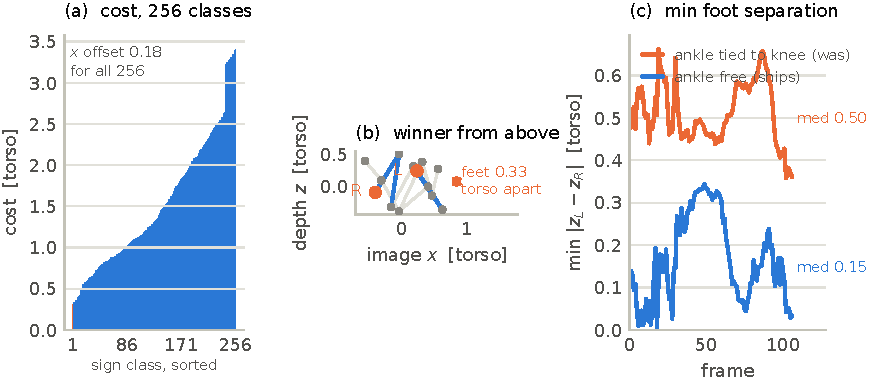
\includegraphics[width=\textwidth]{figures/depth-signs.pdf}
  \caption{The sign search on the example clip, at its deepest frame (46).
  (a) Total cost $\mathcal{C}$ for the $256$ mirror classes, sorted; the winner is
  marked. The horizontal offset is $0.183\,\Lt$ for every one of them, so the ranking is
  purely a depth judgement. (b) That winner seen from above, legs highlighted:
  its feet sit $0.33\,\Lt$ apart in depth, against $1.86$ under the tied rule
  this replaced. (c) Why --- the smallest foot separation any sign assignment
  can reach, per frame. With the ankle's sign tied to the knee's the floor is
  $0.50\,\Lt$ median: the tied search cannot put the feet together at any frame
  of the catch, whatever it scores. Freeing the bit drops the floor to $0.15$.}
  \label{fig:depthsign}
\end{figure}

\subsection{The plate-anchored variant}

When plates are detected the depths are anchored rather than guessed: the
ellipse fit gives $s$ and the 3D bar axis; each wrist is taken to lie on the bar
and inherits the bar's depth beneath its own image position; the remaining
joints are reached by breadth-first propagation with the same $dz$ as
\S\ref{sec:depth-fore}, now in millimetres. This is the only path that produces
absolute lengths. It needs both a plate ellipse and a visible wrist, and falls
back to pinning the pelvis at $z=0$.

\subsection{The tied-sign failure, and what it cost}\label{sec:depth-broken}

Ankles used to inherit the knee's sign and wrists the elbow's, on the argument
that a limb segment follows the segment it hangs off. For a straight limb that
holds. For a flexed one it is backwards: in a squat the thigh runs forward and
down from the hip while the shank runs \emph{backward} and down from the knee,
so the two segments have opposite depth signs. Tying them sends the foot out to
$z_{\text{knee}}+dz_{\text{shank}}$ instead of back under the hip.

The consequence was structural, not a tuning failure.
Fig.~\ref{fig:depthsign}c sweeps every assignment at every frame and keeps the
smallest foot separation each scheme can reach: tied, the median floor is
$0.50\,\Lt$; with the distal signs free it is $0.15\,\Lt$. A feet-together squat
was therefore not merely disfavoured by the search --- it was unreachable, and
the balance criterion was left choosing the least-bad member of a set that did
not contain the answer. The result satisfied every bone length, every joint
angle and the balance test, and put the athlete's feet $1.86\,\Lt$ apart in
depth, roughly a metre, where the video shows them planted side by side.

That is the general shape of the risk here, and it is worth stating plainly: a
cost function can only rank the reconstructions its parameterisation can
express. A good score is evidence about the search, not about the body, and the
two are only the same thing if the truth is in the candidate set. Both fixes in
this appendix --- freeing the distal signs, and scaling off the clip rather than
the frame --- were found by checking a reconstruction against anatomy rather
than against its own objective.

What remains genuinely unresolved is the front/back mirror (\S\ref{sec:depth-sign}):
it is gauge, no image-plane criterion can touch it, and it is left to the user.
The per-joint controls and click-to-flip in the 3D view exist for that. Absolute
depth is still only available on the plate-anchored path; the keypoint lift
remains unit-torso and should be read as a solved sketch, not a measurement.

\begin{thebibliography}{9}\small
\bibitem{vitpose} Y.~Xu, J.~Zhang, Q.~Zhang, D.~Tao. \emph{ViTPose: Simple Vision Transformer Baselines for Human Pose Estimation.} NeurIPS 35, 2022. arXiv:2204.12484. Implementation used: \texttt{github.com/JunkyByte/easy\_ViTPose}.
\bibitem{vit} A.~Dosovitskiy, L.~Beyer, A.~Kolesnikov, D.~Weissenborn, X.~Zhai, T.~Unterthiner, M.~Dehghani, M.~Minderer, G.~Heigold, S.~Gelly, J.~Uszkoreit, N.~Houlsby. \emph{An Image is Worth 16$\times$16 Words: Transformers for Image Recognition at Scale.} ICLR, 2021. arXiv:2010.11929.
\bibitem{mae} K.~He, X.~Chen, S.~Xie, Y.~Li, P.~Doll\'ar, R.~Girshick. \emph{Masked Autoencoders Are Scalable Vision Learners.} CVPR, 2022. arXiv:2111.06377.
\bibitem{yolov8} G.~Jocher, A.~Chaurasia, J.~Qiu. \emph{Ultralytics YOLOv8} (v8.0.0), 2023. \texttt{github.com/ultralytics/ultralytics}.
\bibitem{sort} A.~Bewley, Z.~Ge, L.~Ott, F.~Ramos, B.~Upcroft. \emph{Simple Online and Realtime Tracking.} IEEE ICIP, 2016. arXiv:1602.00763.
\bibitem{fc} F.~N.~Fritsch, R.~E.~Carlson. \emph{Monotone Piecewise Cubic Interpolation.} SIAM J.\ Numer.\ Anal.\ 17(2):238--246, 1980. doi:10.1137/0717021.
\end{thebibliography}

\end{document}
